\documentclass[a4paper,9pt]{extarticle}	%artykuł

\usepackage[utf8]{inputenc}								%kodowanie znaków
\usepackage{inconsolata}								%Consolas font
\usepackage[T1]{fontenc}								%kodowanie fontu
\usepackage{polski}										%polskie wcięcia itp
\usepackage{graphicx}									%wstawianie grafik
\usepackage{booktabs}									%scalanie kolumn
\usepackage{enumitem}									%lista a), b), c)
\usepackage{multirow}									%scalanie komórek tabeli w pionie
\usepackage{listings}									%wklejanie kodu z SQL
\usepackage{xcolor}										%żeby kolory do kodu działaly
\usepackage[margin=0.5in]{geometry}					%zmiana marginesów
\usepackage[hidelinks]{hyperref}						%linki w spisie treści

\hypersetup{linktoc=all}								%ustawienie linków w spisie treści
\linespread{1.3}										%interlinia 1,5

%\renewcommand\familydefault{\sfdefault}

\lstset{ %
  backgroundcolor=\color{white},   % choose the background color; you must add \usepackage{color} or \usepackage{xcolor}; should come as last argument
  basicstyle=\ttfamily,        % the size of the fonts that are used for the code
  breakatwhitespace=false,         % sets if automatic breaks should only happen at whitespace
  breaklines=true,                 % sets automatic line breaking
  commentstyle=\color{gray},    	% comment style
  extendedchars=true,              % lets you use non-ASCII characters; for 8-bits encodings only, does not work with UTF-8
  frame=single,	                    % adds a frame around the code
  keywordstyle=\color{blue},       % keyword style
  language=Java,             % the language of the code
  morekeywords={*,...},            % if you want to add more keywords to the set
%  numbers=left,                    % where to put the line-numbers; possible values are (none, left, right)
%  numbersep=5pt,                   % how far the line-numbers are from the code
%  numberstyle=\normalsize,			% the style that is used for the line-numbers
  rulecolor=\color{black},         % if not set, the frame-color may be changed on line-breaks within not-black text (e.g. comments (green here))
  showspaces=false,                % show spaces everywhere adding particular underscores; it overrides 'showstringspaces'
  showstringspaces=false,          % underline spaces within strings only
  showtabs=false,                  % show tabs within strings adding particular underscores
  stepnumber=1,                    % the step between two line-numbers. If it's 1, each line will be numbered
  stringstyle=\color{orange},      % string literal style
  tabsize=2	                  		% sets default tabsize to 2 spaces                   
}

\lstset{language=Java,
       }

\lstset{
literate=%
{ą}{{\k{a}}}1
{Ą}{{\k{A}}}1
{ć}{{\'c}}1
{Ć}{{\'{C}}}1
{ę}{{\k{e}}}1
{Ę}{{\k{E}}}1
{ł}{{\l{}}}1
{Ł}{{\L{}}}1
{ń}{{\'n}}1
{Ń}{{\'N}}1
{ó}{{\'o}}1
{Ó}{{\'O}}1
{ś}{{\'s}}1
{Ś}{{\'S}}1
{ż}{{\.z}}1
{Ż}{{\.Z}}1
{ź}{{\'z}}1
{Ź}{{\'Z}}1
}

\begin{document}

\begin{center}

{\LARGE \textbf{Bazy danych \ppauza NoSQL}}


{\Large \textbf{Neo4j \ppauza zadania}}

\end{center}

Autor zadań: Piotr Wróbel

Data laboratorium: 4.12.2019 r.

Data wykonania: 9.01.2020 r.

\begin{enumerate}
  \item Zaimplementować funkcję \ppauza zaimplementowano przykładowe zapytanie MATCH zwracające tytuły filmów zawierające wyraz ,,You'', kod w Javie przedstawiono poniżej, a~wynik wywołania na Rysunku~\ref{scrn:1}:
  \begin{lstlisting}
public class Main {

    static Connection connection;

    public static void main(String[] args) {
        try {
            connection = DriverManager.getConnection("jdbc:neo4j:http://localhost:7474", "neo4j", "mojeHasło");
            exampleMatch();
            connection.close();
        } catch (SQLException e) {
            e.printStackTrace();
        }
    }

    public static void exampleMatch() throws SQLException {
        String query = "MATCH (m:Movie) WHERE m.title CONTAINS 'You' RETURN m.title";
        PreparedStatement statement = connection.prepareStatement(query);
        ResultSet rs = statement.executeQuery();
        while(rs.next()){
            System.out.println("Movie: " + rs.getString("m.title"));
        }

        statement.close();
        rs.close();
    }
}
  \end{lstlisting}
  
  \begin{figure}[ht]
    \centering
    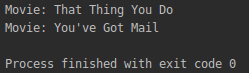
\includegraphics[scale=0.5]{screeny/1.png}
    \caption{Wynik wywołania przykładowego polecenia MATCH z~poziomu Javy}
    \label{scrn:1}
  \end{figure}
  
  \item Stworzyć kilka nowych węzły reprezentujących film oraz aktorów w nim występujących, następnie stworzyć relacje ich łączące (np. ACTED\_IN).
  Utworzono węzeł odpowiadający filmowi i~węzły trzech aktorów w~nim grających, użyty kod przedstawiono poniżej, a~wizualizację wyniku na Rysunku~\ref{scrn:2}
  \begin{lstlisting}
CREATE (m:Person { name: 'Daisy Ridley' })
CREATE (m:Person { name: 'Adam Driver' })
CREATE (m:Person { name: 'John Boyega' })
CREATE (m:Movie { title: 'Star Wars: The rise of Skywalker' })
MATCH (a:Person), (m:Movie) WHERE a.name = 'Daisy Ridley' AND m.title = 'Star Wars: The rise of Skywalker' CREATE (a)-[r:ACTED_IN]->(m)
MATCH (a:Person), (m:Movie) WHERE a.name = 'Adam Driver' AND m.title = 'Star Wars: The rise of Skywalker'  CREATE (a)-[r:ACTED_IN]->(m)
MATCH (a:Person), (m:Movie) WHERE a.name = 'John Boyega' AND m.title = 'Star Wars: The rise of Skywalker'  CREATE (a)-[r:ACTED_IN]->(m)
  \end{lstlisting}
  
  \begin{figure}[ht]
    \centering
    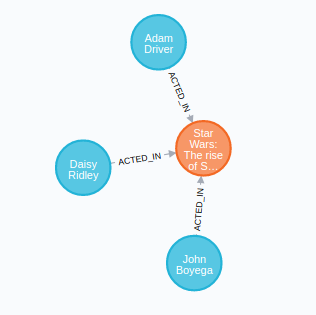
\includegraphics[scale=0.5]{screeny/2.png}
    \caption{Utworzone nowe węzły bazy}
    \label{scrn:2}
  \end{figure}
  
  \item Dodać zapytaniem nowe właściwości nowo dodanych węzłów reprezentujących aktor (np. \textit{birthdate}
oraz \textit{birthplace}). Zapytania przedstawiono poniżej, a efekt na Rysunku~\ref{scrn:3}
	\begin{lstlisting}
MATCH (a:Person) WHERE a.name = 'Daisy Ridley' SET a.birthplace = 'Londyn', a.birthdate = '10-04-1992'
MATCH (a:Person) WHERE a.name = 'Adam Driver' SET a.birthplace = 'San Diego', a.birthdate = '19-11-1983'
MATCH (a:Person) WHERE a.name = 'John Boyega' SET a.birthplace = 'Londyn', a.birthdate = '17-03-1992'
  \end{lstlisting}
  
  \begin{figure}[ht]
    \centering
    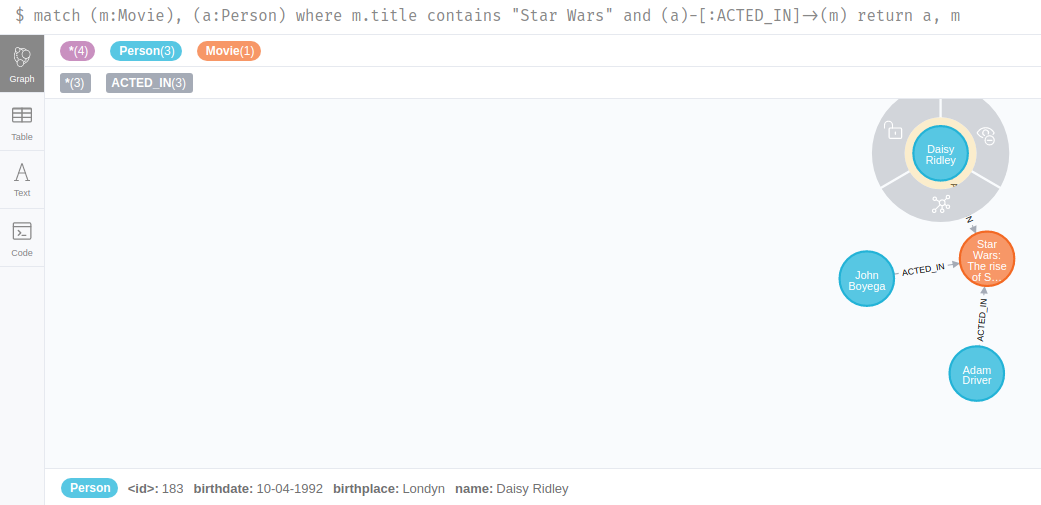
\includegraphics[width=0.9\textwidth]{screeny/3.png}
    \caption{Efekt dodania wartości atrybutów \textit{birthplace} i \textit{birthdate} dla aktorów.}
    \label{scrn:3}
  \end{figure}
  
  \item Ułożyć zapytanie, które zmieni wartość atrybutu węzłów danego typu, jeżeli innych atrybut węzła
spełnia zadane kryterium.
  Ułożono zapytanie, które zmienia wartość atrybutu \textit{tagline} na ,,nowy tagline'' dla filmów wydanych w~roku 1996 (efekt wywołania przedstawia Rysunek~\ref{scrn:4}):
  \begin{lstlisting}
MATCH (m:Movie) WHERE m.released = 1996 SET m.tagline = 'nowy tagline' RETURN m
  \end{lstlisting}
\newpage  
  \begin{figure}[ht]
    \centering
    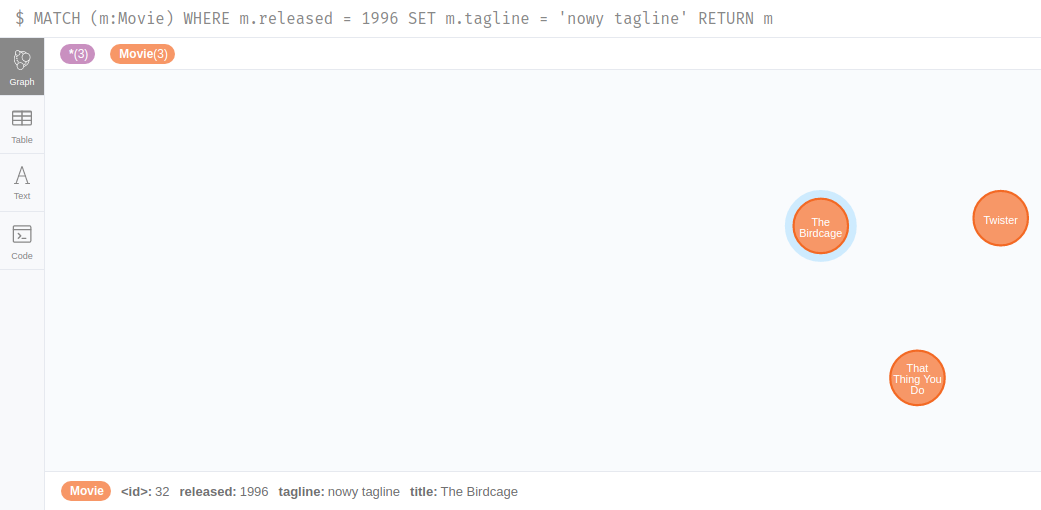
\includegraphics[width=0.9\textwidth]{screeny/4.png}
    \caption{Efekt modyfikacji atrybutu \textit{tagline} dla filmów wydanych w 1996 roku.}
    \label{scrn:4}
  \end{figure}
  
  \item Zapytanie o aktorów którzy grali w conajmniej 2 filmach (użyć collect i length) (Rysunek~\ref{scrn:5a}):
  \begin{lstlisting}
  MATCH (p:Person)-[r:ACTED_IN]->(m:Movie) WITH p, length(collect(r)) AS films WHERE films >= 2  return p
  \end{lstlisting}  
  \begin{figure}[ht]
    \centering
    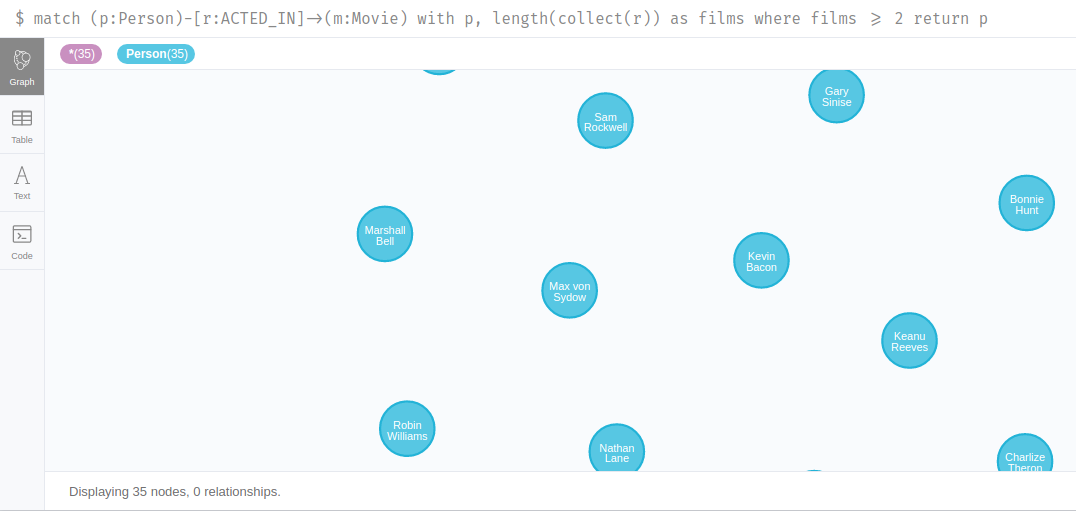
\includegraphics[width=0.9\textwidth]{screeny/5a.png}
    \caption{Efekt wyszukania aktorów, którzy grali w~conajmniej 2~filmach.}
    \label{scrn:5a}
  \end{figure}
  
   i policzyć średnią wystąpień w filmach dla grupy aktorów, którzy wystąpili w conajmniej 3 filmach (Rysunek~\ref{scrn:5b}):
   \begin{lstlisting}
   match (p:Person)-[r:ACTED_IN]->(m:Movie) with p, length(collect(r)) as films where films >= 3  return avg(films)
   \end{lstlisting}
   \begin{figure}[ht]
    \centering
    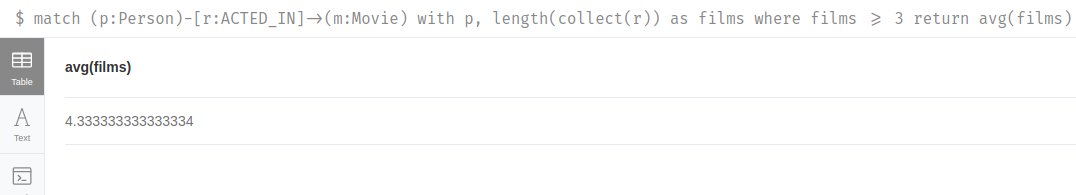
\includegraphics[width=0.9\textwidth]{screeny/5b.png}
    \caption{Średnia ilości ról dla aktorów, którzy grali w~conajmniej 3~filmach.}
    \label{scrn:5b}
  \end{figure}
   
   \newpage
  \item Zmienić wartość wybranego atrybutu w węzłach na ścieżce pomiędzy dwoma podanymi węzłami (wynik - Rysunek~\ref{scrn:6}):
  \begin{lstlisting}
  match (p:Person)-[r:ACTED_IN]->(m:Movie) where p.name = 'Rita Wilson' and m.title contains 'Sleepless' set r.roles = 'zmiana roli' return p, r, m
  \end{lstlisting}
  \begin{figure}[ht]
    \centering
    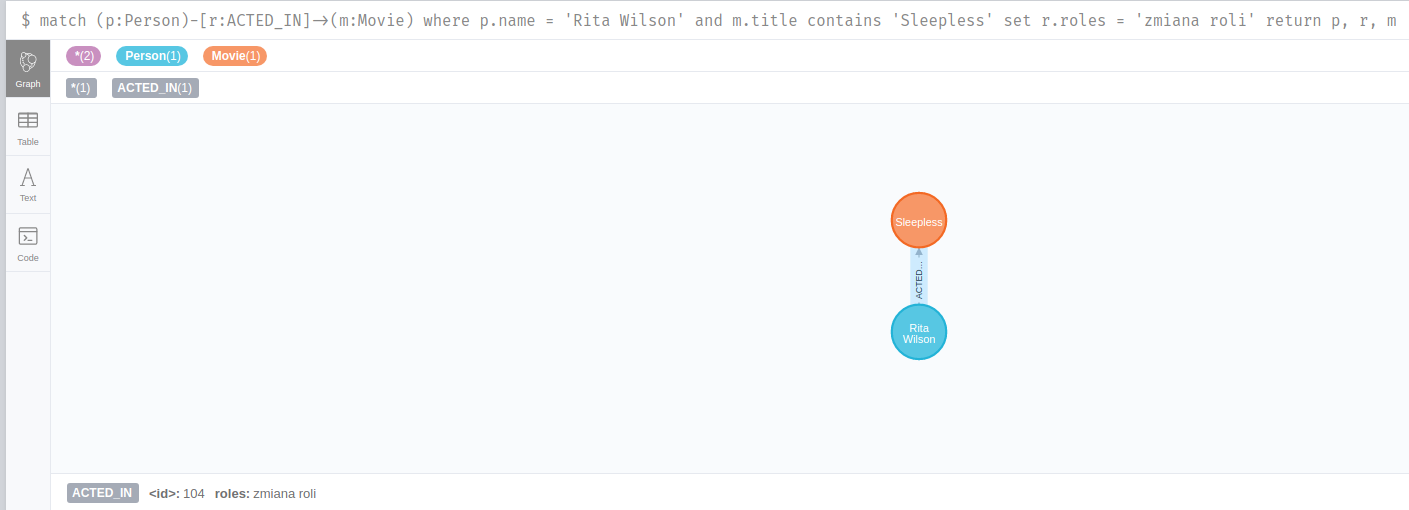
\includegraphics[width=0.9\textwidth]{screeny/6.png}
    \caption{Efekt zmiany wartości atrybutu relacji.}
    \label{scrn:6}
  \end{figure}
  
  \item Wyświetlić węzły, które znajdują się na 2 miejscu na ścieżkach o długości 4 pomiędzy dwoma wybranymi węzłami (Rysunek~\ref{scrn:7}).
  \begin{lstlisting}
  match p = (a:Person)-[*4]-(b:Person) where a.name contains 'Keanu Reeves' and b.name contains 'Milos Forman' return nodes(p)[2]
  \end{lstlisting}
  \begin{figure}[ht]
    \centering
    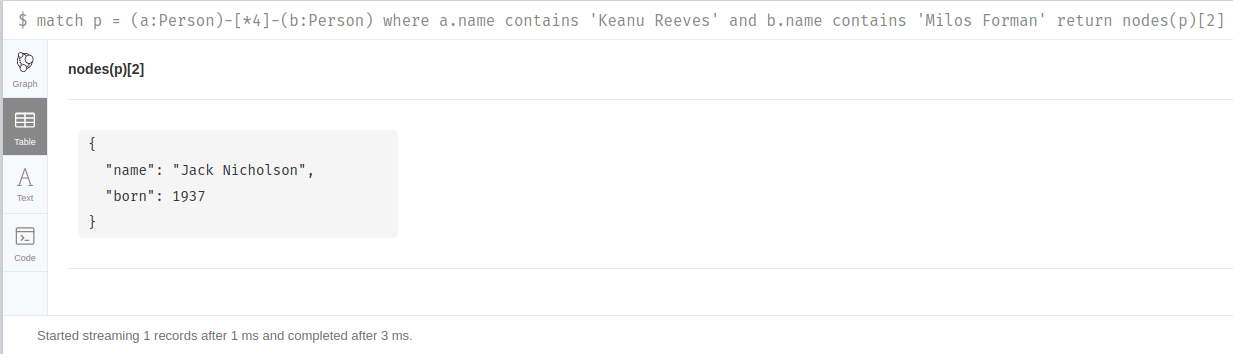
\includegraphics[width=0.9\textwidth]{screeny/7.png}
    \caption{Drugi element 4-elementowej ścieżki.}
    \label{scrn:7}
  \end{figure}
\newpage
  \item Porównać czas wykonania zapytania o wybranego aktora bez oraz z indeksem w bazie nałożonym na atrybut name (DROP INDEX i CREATE INDEX oraz użyć komendy PROFILE/EXPLAIN).
  \begin{itemize}
  \item Wynik szukania bez indeksu \ppauza Rysunek~\ref{scrn:8a}
   \begin{figure}[ht]
    \centering
    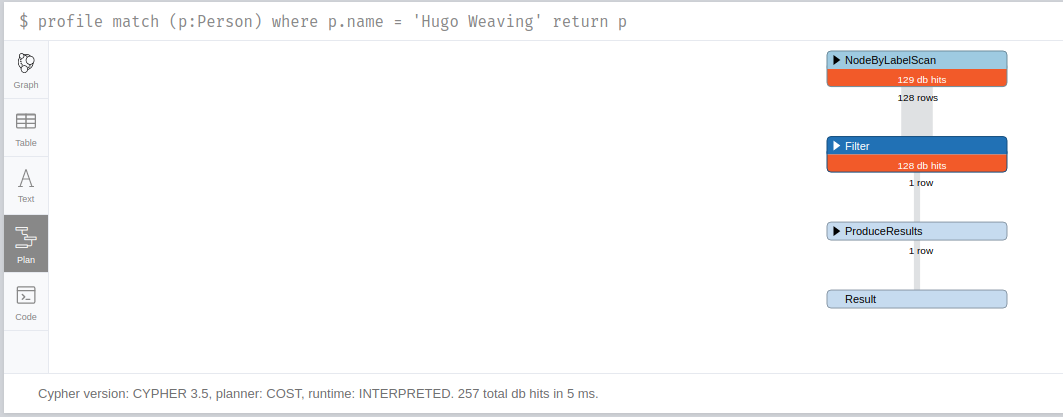
\includegraphics[width=0.9\textwidth]{screeny/8a.png}
    \caption{Wyszukiwanie aktora po imieniu bez założonego indeksu.}
    \label{scrn:8a}
  \end{figure}
  \item Wynik szukania z~indeksem \ppauza Rysunek~\ref{scrn:8b}
  \end{itemize}
  \begin{figure}[ht]
    \centering
    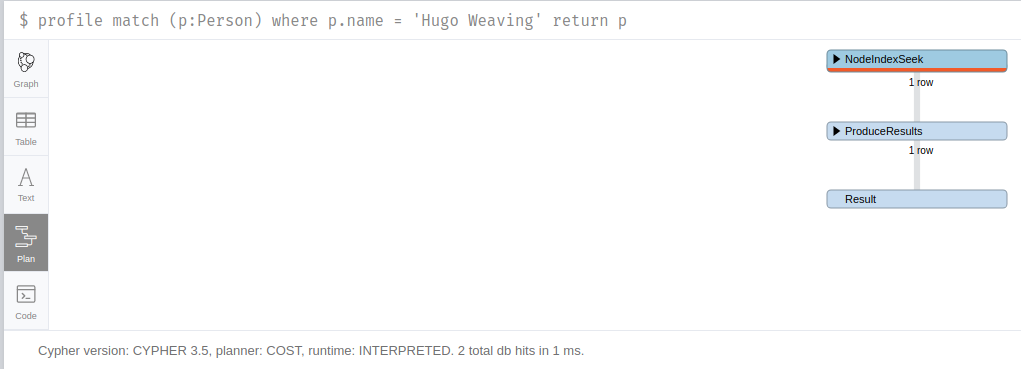
\includegraphics[width=0.9\textwidth]{screeny/8b.png}
    \caption{Wyszukiwanie aktora po imieniu z założonym indeksem.}
    \label{scrn:8b}
  \end{figure}

 \newpage 
  \item Spróbować dokonać optymalizacji wybranych dwóch zapytań z poprzednich zadań
    \begin{itemize}
      \item efekt założenia indeksu na atrybut name dla polecenia wyswietlenia węzłów na 2 miejscu ścieżki o długości 4 \ppauza wyniki Rysunek~\ref{scrn:9a} i~\ref{scrn:9b}
  \begin{figure}[ht]
    \centering
    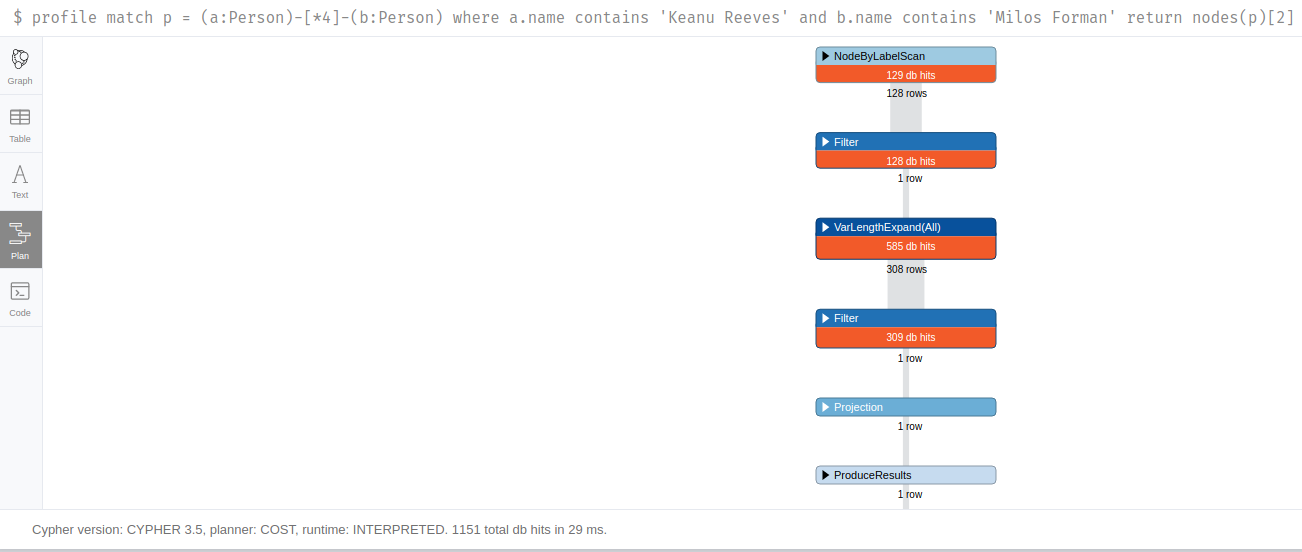
\includegraphics[width=0.9\textwidth]{screeny/9a.png}
    \caption{Drugi element 4\dywiz{}elementowej ścieżki bez założonego indeksu.}
    \label{scrn:9a}
  \end{figure}
  
  \begin{figure}[ht]
    \centering
    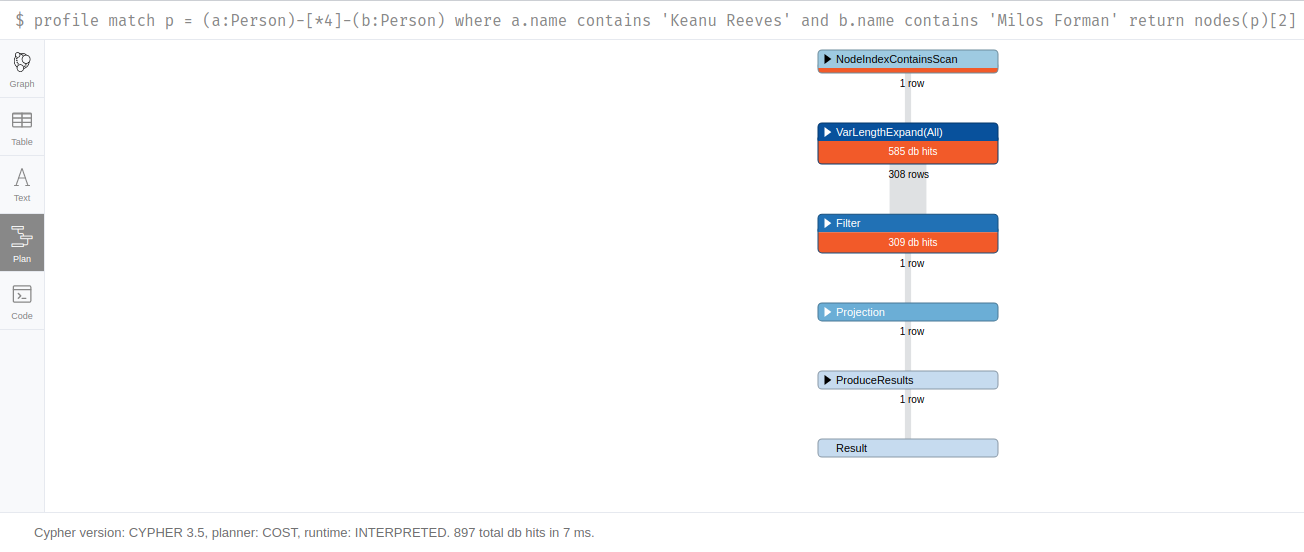
\includegraphics[width=0.9\textwidth]{screeny/9b.png}
    \caption{Drugi element 4\dywiz{}elementowej ścieżki z założonym indeksem.}
    \label{scrn:9b}
  \end{figure}
      
\newpage   
      \item efekt założenia indeksu na atrybuty released i tagline filmu dla zapytania z punktu, w~którym zmieniano wartość atrybutu węzłów \ppauza wyniki Rysunek~\ref{scrn:9c} i~\ref{scrn:9d}.
  \begin{figure}[ht]
    \centering
    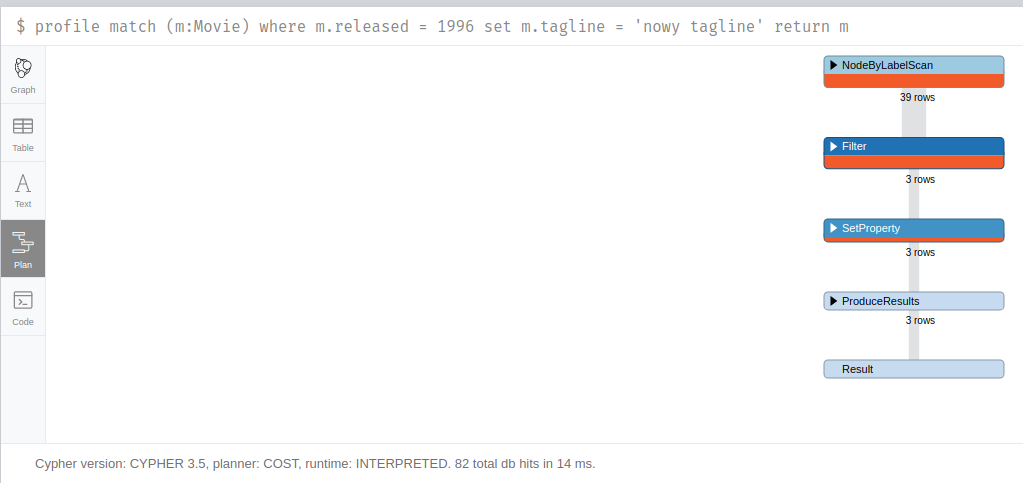
\includegraphics[width=0.9\textwidth]{screeny/9c.png}
    \caption{Zmiana atrybutu filmów bez indeksu na atrybucie \textit{released}.}
    \label{scrn:9c}
  \end{figure}
  \begin{figure}[ht]
    \centering
    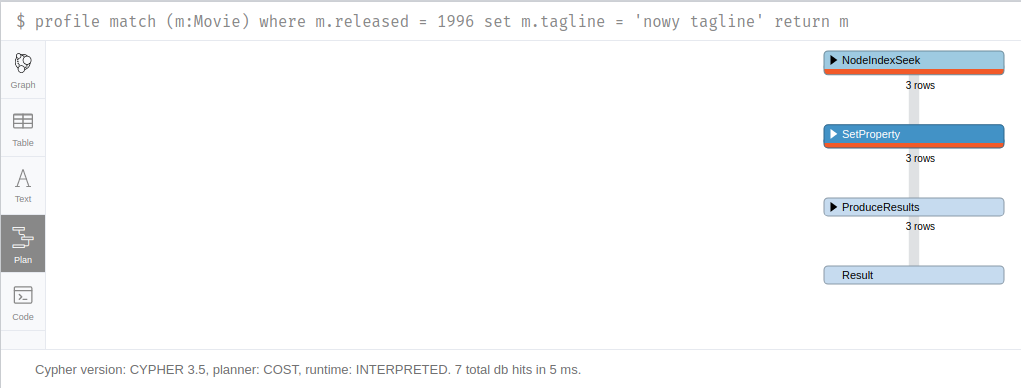
\includegraphics[width=0.9\textwidth]{screeny/9d.png}
    \caption{Zmiana atrybutu filmów z indeksem na atrybucie \textit{released}.}
    \label{scrn:9d}
  \end{figure}      
    \end{itemize}

\newpage
\item Napisać kod, które wygeneruje drzewo rozpinające z bazy

\begin{figure}[ht]
  \centering
  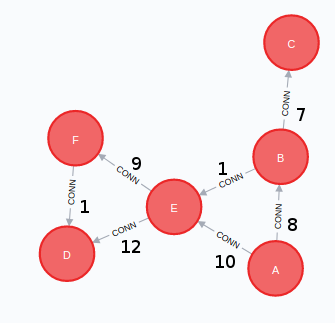
\includegraphics[scale=0.5]{screeny/10a.png}
  \caption{Graf użyty w zadaniu, do krawędzi dopisano ich koszty}
  \label{scrn:10a}
\end{figure}

Wygenerowano przykładowy mały graf skierowany o strukturze przedstawionej na Rysunku~\ref{scrn:10a} (nad krawędziami pokazane są koszty połączeń). W bazie danych każdy wierzchołek ma typ Edge, właściwość label, a~każda relacja jest rodzaju CONN i ma właściwości cost i mst (mst jest pomocnicza do wyznaczenia drzewa rozpinającego). 

Przykładowe zapytania dodające dane do bazy:
\begin{lstlisting}
CREATE (a:Elem { label = 'A' })
MATCH (a:Elem), (b:Elem) where a.label = 'A' AND b.label = 'B' CREATE (a)-[:CONN]->(b)
match (a:Elem)-[e:CONN]->(b:Elem) where a.label = 'A' AND b.label = 'B' set e.cost = 8
\end{lstlisting}

W~Javie wierzchołki są reprezentowane przez klasę Node:
\begin{lstlisting}
public class Node {
    private String label;
    private Set<Edge> neighbours;

    public Node(String label) {
        this.label = label;
        this.neighbours = new HashSet<>();
    }

    public String getLabel() {
        return label;
    }

    public Set<Edge> getNeighbours() {
        return neighbours;
    }

    public void addEdge(Edge edge) {
        this.neighbours.add(edge);
    }

    @Override
    public boolean equals(Object o) {
        if (this == o) return true;
        if (o == null || getClass() != o.getClass()) return false;
        Node node = (Node) o;
        return label.equals(node.label);
    }

    @Override
    public int hashCode() {
        return Objects.hash(label);
    }
}
\end{lstlisting}

a~krawędzie przez klasę Edge:
\begin{lstlisting}
public class Edge implements Comparable<Edge> {
    private Node start;
    private Node stop;
    private int cost;

    public Edge(Node start, Node stop, int cost) {
        this.start = start;
        this.stop = stop;
        this.cost = cost;

        start.addEdge(this);
    }

    public Node getStart() {
        return start;
    }

    public Node getStop() {
        return stop;
    }

    public int getCost() {
        return cost;
    }

    @Override
    public int compareTo(Edge o) {
        return this.cost - o.getCost();
    }

    @Override
    public boolean equals(Object o) {
        if (this == o) return true;
        if (o == null || getClass() != o.getClass()) return false;
        Edge edge = (Edge) o;
        return cost == edge.cost &&
                start.equals(edge.start) &&
                stop.equals(edge.stop);
    }

    @Override
    public int hashCode() {
        return Objects.hash(start, stop, cost);
    }
}
\end{lstlisting}

W głównej funkcji programu najpierw czytane są z bazy dane o wierzchołkach i krawędziach, a~następnie jest tworzone minimalne drzewo rozpinające z użyciem algorytmu Prima. Krawędzie należące do drzewa mają zmieniony atrybut mst na wartość 1. Kod głównej klasy:
\begin{lstlisting}
public class Main {

    static Connection connection;

    public static void main(String[] args) {
        try {
            connection = DriverManager.getConnection("jdbc:neo4j:http://localhost:7474", "neo4j", "mojeHasło");

            List<Node> nodes = new LinkedList<>();
            readNodes(nodes);
            readEdges(nodes);

            int indexOfA = nodes.indexOf(new Node("A"));
            Node startingNode = nodes.get(indexOfA);
            nodes.remove(startingNode);

            PriorityQueue<Edge> edgesQueue = new PriorityQueue<>(startingNode.getNeighbours());
            while(!nodes.isEmpty()) {
                Edge nextEdge = edgesQueue.poll();
                if(nodes.contains(nextEdge.getStop())) {
                    Node stopNode = nextEdge.getStop();
                    nodes.remove(stopNode);
                    edgesQueue.addAll(stopNode.getNeighbours());
                    markEdge(nextEdge);
                }
            }

            connection.close();
        } catch (SQLException e) {
            e.printStackTrace();
        }
    }

    public static void markEdge(Edge edge) throws SQLException {
        String query = String.format("MATCH (a:Elem)-[r:CONN]->(b:Elem) WHERE a.label = '%s' AND b.label = '%s' SET r.mst = 1",
                edge.getStart().getLabel(), edge.getStop().getLabel());
        Statement statement = connection.createStatement();
        statement.execute(query);
    }

    public static void readNodes(List<Node> nodes) throws SQLException {
        String query = "MATCH (e:Elem) RETURN e.label";
        PreparedStatement statement = connection.prepareStatement(query);
        ResultSet rs = statement.executeQuery();

        while(rs.next()) {
            nodes.add(new Node(rs.getString("e.label")));
        }
    }

    public static void readEdges(List<Node> nodes) throws SQLException {
        String query = "match (a:Elem)-[r:CONN]->(b:Elem) return a.label, b.label, r.cost";
        PreparedStatement statement = connection.prepareStatement(query);
        ResultSet rs = statement.executeQuery();

        while(rs.next()) {
            int startIndex = nodes.indexOf(new Node(rs.getString("a.label")));
            Node start = nodes.get(startIndex);

            int stopIndex = nodes.indexOf(new Node(rs.getString("b.label")));
            Node stop = nodes.get(stopIndex);

            Edge edge = new Edge(start, stop, rs.getInt("r.cost"));
        }
    }
}
\end{lstlisting}

W~celu wygodnej wizualizacji uzyskanego drzewa, usunięto z~bazy krawędzie które do drzewa nie należą i~wywołano odpowiednie zapytanie MATCH \ppauza wynik przedstawia Rysunek~\ref{scrn:10b}.

\begin{figure}[ht]
  \centering
  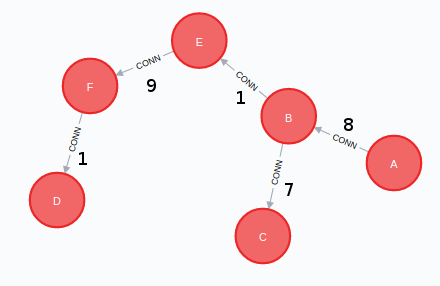
\includegraphics[scale=0.5]{screeny/10b.png}
  \caption{Minimalne drzewo rozpinające, do krawędzi dopisano ich koszty}
  \label{scrn:10b}
\end{figure}

\end{enumerate}

\end{document}